\chapter{Pesquisa de Referências}

Este capítulo apresenta as referências utilizadas para poder avaliar a aplicação de uma rede neural artificial para generalizar as principais equações encontradas na literatura. Apresenta uma breve explicação de como as precipitações são formadas e quais instrumentos são utilizados para realizar as medições das chuvas. 

\section{Formação das precipitações}

De acordo com (MARENGO, 2008), a superfície terrestre está coberta em sua maior parte por água, este elemento representa 70\% da superfície da Terra estando sempre em constante movimento. A água é um elemento básico para a sobrevivência de todos os organismos vivos, pode-se encontrar a água nos três estados da matéria (sólido, líquido e gasoso), sendo possível observar as três fases no ciclo hidrológico (TUNDISI, 2003).

O ciclo hidrológico é o movimento contínuo da água presente nos oceanos, continentes e na atmosfera, é o grande responsável pela distribuição e disponibilidade de água no planeta. Os principais processos que envolvem o ciclo hidrológico são: precipitação, interceptação, evaporação, transpiração, infiltração, percolação e escoamento superficial (TUNDISI, 2003).

A definição do regime hidrológico ocorre pela combinação das características físicas de cada região (geologia, topografia e clima) e da ação do ciclo hidrológico. Assim sendo, existe uma desigualdade na distribuição de água, espacialmente e temporalmente, o que leva à necessidade de ações de planejamento ambiental de acordo com a situação de excesso ou escassez (TUNDISI, 2003).

A chuva pode ser definida como a precipitação de partículas de água líquida sob a forma de gotas de diâmetro superior a 0,5 mm (MACHADO e TORRES, 2012). As precipitações pluviais podem ser classificadas, conforme a sua origem, de acordo com o mecanismo de ascensão do ar úmido que proporciona a formação das nuvens, sendo que os principais tipos são: ciclônicas (frontais e não frontais), orográficas ou de relevo e convectivas ou de convecção (MIRANDA, OLIVEIRA e SILVA, 2010).

O encontro de massas de ar com propriedades diferentes originam as precipitações ciclônicas, sendo classificadas como frontais e não frontais. As precipitações não frontais podem ser geradas devido à queda de pressão, resultando na elevação do ar em razão da convergência horizontal em áreas de baixa pressão. As chuvas frontais ocorrem, quando a frente fria invade o local, empurrando, para cima, o ar quente e úmido, provocando resfriamento e condensação. São chuvas de grandes durações, abrangem grandes área e de intensidade média (TUCCI, 1993).

As precipitações orográficas (também nomeadas de chuvas de relevo), ocorrem durante a ascensão de massa de ar quente e úmido, pelo encontro de um obstáculo (serras são um exemplo) forçando a elevar-se e, consequentemente, reduzindo a temperatura sucedendo a condensação. Este tipo de chuva ocorre em pequenas áreas, sendo de baixa intensidade e extensa duração (MIRANDA, OLIVEIRA e SILVA, 2010). Após a ocorrência da precipitação, algumas vezes, a massa de ar consegue transpor a barreira, projetando a sombra pluviométrica, caracterizada por regiões secas, devido à umidade já ter sido, em grande parte, descarregada no lado oposto (FORGIARINI, VENDRUSCOLO e RIZZI, 2014).

\textit{Na classificação de precipitações convectivas, enquadram-se as chuvas intensas, típicas de regiões tropicais. A superfície aquecida, desigualmente, forma camadas de ar com densidades diferentes se mantendo em equilíbrio instável. Com a quebra desse equilíbrio (vento, superaquecimento), ocorre a ascensão brusca do ar menos denso, capaz de alcançar grandes altitudes, que atinge o nível de condensação e precipita (VILLELA e MATOS, 1975).}

\section{Medição da chuva}

\subsection{Pluviômetro}
As medições das precipitações de chuvas são realizadas com a utilização de um pluviômetro (Figura 1), aparelho com medidas normalizadas em formato cilíndrico que, exposto às intempéries, reserva a água da chuva precipitada entre um intervalo de leituras. Uma proveta graduada permite a leitura do volume de água acumulado dentro do medidor. O volume de água, dividido pela área de captação do pluviômetro, resulta em uma altura análoga de chuva, definida em milímetros. As leituras devem ser realizadas diariamente, sempre no mesmo horário \cite{manual-daee}.

\begin{figure}[H]
    \caption{Representação do pluviômetro}
    \centering
    \includegraphics[width=0.25\textwidth]{Textuais/Figuras/pluviometro.jpg}
    \fonte{Autores}
    \label{fig:pluviometro}
\end{figure}


\subsection{Pluviógrafo}

Outro tipo de medidor de chuvas é o Pluviógrafo (Figura 2). Existe uma grande variedade de aparelhos, usando princípios diferentes para medir e gravar continuamente as chuvas. Os pluviógrafos permitem medir as intensidades das chuvas durante intervalos de tempo àqueles obtidos com as observações manuais feitas nos pluviômetros \cite{tucci1993}.

\begin{figure}[H]
    \caption{Representação do pluviógrafo}
    \centering
    \includegraphics[width=0.5\textwidth]{Textuais/Figuras/pluviografo.jpg}
    \fonte{Autores}
    \label{fig:pluviografo}
\end{figure}

\section{Dados de chuvas no Brasil}

A Agência Nacional de Águas (ANA) disponibilizada uma relação dos postos pluviométricos instalados e operandos em todo o território brasileiro e os respectivos dados de chuva. Estas informações podem ser obtidas pela Internet por meio do Sistema de Informações Hidrológicas (HidroWeb). 

É importante destacar que, deve-se conhecer a qualidade dos dados que estão sendo utilizados, pois isso pode avariar a qualidade dos resultados dos estudos hidrológicos. Tratando-se de projetos em área urbana, recomenda-se que seja instalado ao menos um pluviógrafo, para aumentar a qualidade dos estudos hidrológicos que apoiarão, por exemplo, os projetos de controle de inundação \cite{tucci1993}.

\section{Caracterização das chuvas intensas}

A intensidade máxima média de precipitação cresce à medida que aumenta o período de retorno, sendo diretamente proporcionais, e decresce com o aumento da duração do evento, sendo inversamente proporcional a duração \cite{analise-chuva}. A principal forma de caracterização de chuvas intensas é por intermédio das equações de intensidade, duração e frequência da precipitação pluvial (equações IDF), ou equações de chuvas intensas \cite{tucci1993}, mais comumente representadas na forma da Equação \ref{eq:equacao-geral}. Estas equações são uma das ferramentas mais utilizadas nos trabalhos de engenharia relacionadas a recursos hídricos \cite{desagregacao}.

\begin{equation}
\label{eq:equacao-geral}
    i = \frac{k \times T_r^a}{(t+b)^c}
\end{equation}

Em que:

i = Intensidade máxima média de precipitação  $[mm.h^-1]$ 

$T_r$ = Período de retorno [anos]

t = Duração [min]

K, a, b, c = Parâmetros de ajuste estatístico, referentes à cada localidade

Para cada localidade ou plataforma de coleta de dados é feito, individualmente, o ajuste da equação para chuvas intensas. Recomenda-se ser feito com a utilização de um extenso período de dados, constituída de pluviógrafos \cite{interpolacao-chuva} apropriado a cada precipitação específica ocorrida em um posto pluviométrico, durante anos de observação. Entretanto, tais pluviógrafos dificilmente são disponíveis em quantidade e qualidade apropriada, devido à baixa densidade de equipamentos registradores espalhados no país, e às séries disponíveis serem frequentemente curtas e com falhas nos registros \cite{relacao-precipitacao}.

O estabelecimento de cada equação utiliza metodologia de exaustivo trabalho de tabulação, análise e interpretação de grande quantidade de pluviogramas, fitas utilizadas no registro por pluviógrafos \cite{relacao-precipitacao}. 

Decorrente da dificuldade de obtenção dos dados pluviográficos, a grande parte dos estudos realizados no Brasil, são efetuados com séries históricas inferiores à recomendada \cite{variabilidade-espacial}. A Organização Mundial de Meteorologia (OMM) recomenda a adoção de série histórica de no mínimo 30 anos.

Na prática, é difícil fixar o valor de intensidade da chuva, uma vez que o impacto é variável de local para local, seja em área rural ou urbana \cite{hidro-basica}. Em países subdesenvolvidos, as redes de dados climatológicos existentes são esparsas e escassas, reflexo na má qualidade dos projetos, originando obras sub ou superestimadas, quando superestimadas, podem gerar um desperdício econômico; e quando subestimadas, uma redução da confiabilidade de eficiência da obra e aumento do risco \cite{tucci1993}. Por esta razão, há barreiras na realização de projetos de obras hidráulicas mais confiáveis e econômicos \cite{chuva-bahia}. 

A busca por uma associação intensidade-duração-frequência de uma chuva é anterior a 1932 \cite{desagregacao}. Desde 1960 países desenvolvidos tem estudado a sua distribuição geográfica, onde possuem mapas que fornecem as intensidades e alturas de precipitação \cite{desagregacao}. Os estudos pioneiros no Brasil foram desenvolvidos por Pfafstetter (1957) e Denardin e Freitas (1982), em que Denardin e Freitas (1982) ajustaram equações matemáticas, a partir de gráficos apresentados por Pfafstetter (1957), que possibilitaram cálculo das alturas pluviométricas, em função da duração da precipitação e do período de retorno, por meio do método de regressão não-linear múltipla, para 80 estações pluviográficas distribuídas para todo o país \cite{relacao-idf-nordeste}.

No caso de não se ter informações provenientes de pluviogramas para determinar a equação de chuvas intensas, sendo a situação mais comum, existem alternativas para criação de informações das chuvas intensas \cite{interpolacao-chuva}. \citeonline{artigo-chuva} indicam a utilização de equações de regiões próximas, reduzindo a probabilidade de afetar a confiabilidade da estimativa. Outra alternativa bastante comum é a utilização de dados pluviométricos de captação diários, adquiridos de estação para estimar as equações, com a aplicação de métodos para desagregação de chuvas \cite{idf-rs}, o qual aproxima intensidades para durações inferiores a um dia \cite{relacoes-sc}. Finalmente, uma alternativa que vem ganhando espaço para a estimação dos parâmetros das equações de chuvas intensas em localidades sem qualquer registro de chuva consiste no uso de técnicas de interpolação espacial \cite{chuva-bahia}.

\begin{figure}[H]
    \caption{Representação das equações IDF}
    \centering
    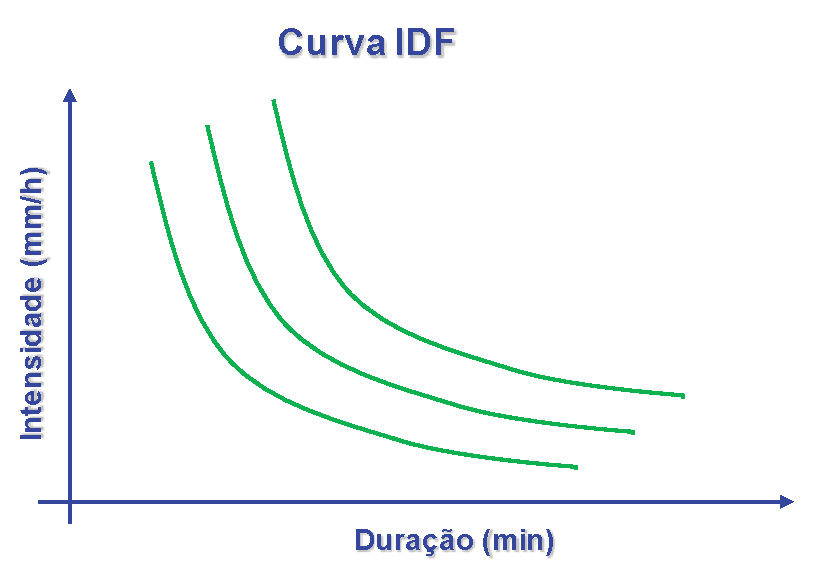
\includegraphics[width=0.8\textwidth]{Textuais/Figuras/curva-idf.pdf}
    \fonte{Autores}
    \label{fig:desagregacao}
\end{figure}

\section{Modelos matemáticos que expressam a relação IDF}

As relações intensidade-duração-frequência podem ser expressas matematicamente, ou seja, equações propostas que representam a quantidade máxima de uma chuva. A definição do modelo que representa as chuvas intensas, utilizado em cada trabalho, deve ser de fácil manuseio, mantendo a segurança em seus resultados que devem ser o mais próximo à realidade (MELLO, LIMA e MELLO, 2003).

Segundo Villela e Mattos (1975), o modelo matemático clássico mais utilizado é expresso pela Equação 1.

Em situações onde a escassez de dados é muito grande, (MELLO, LIMA e MELLO, 2003) evidenciam a importância da comparação entre vários modelos que representam a relação IDF, podendo resultar em informações confiáveis e precisas. Em seu trabalho, os autores, utilizam modelos exponencial e linear (Equação 2 e 3).

Mello et al. (2003) concluíram que o modelo exponencial produziu erros menores, gerando melhores aproximações da intensidade máxima de chuvas. O modelo linear, apesar de possuir um coeficiente de determinação $r^2$ superior a 0,99, não foi considerado confiável para utilização em estudos de chuvas intensas pois apresenta os maiores erros médios e, também, a maior amplitude de erros comparado ao modelo exponencial.

Pfafstetter (1957), em seu trabalho de determinação das curvas IDF, realizou o ajuste do modelo representado pela Equação 4.

A Equação 4 fornece a precipitação para período de retorno de 1 ano e a Equação 5 permite estimar a chuva para outros tempos de retorno (TUCCI, 2004).

Bertoni e Tucci (2001) detalharam a metodologia de Bell, que relaciona a precipitação máxima para um tempo de duração definido e período de retorno a uma precipitação padrão de 60 min de duração e 2 anos de período de retorno (Equação 6).

Se acordo com Sampaio (2011), a metodologia Bell se baseia em séries de chuva, observados em todo globo terrestre, destacando que o valor máximo das chuvas está relacionando a regiões convectivas com características parecidas no mundo todo; assinalando isso com uma desvantagem do método, uma vez que as equações são geradas de valores médias e não específicos para uma determinada região. O autor, também, apontou como desvantagem que o valor da precipitação máxima obtida é válido apenas para durações entre 5 a 120 min.
Mello et al. (2003) comentaram que a principal característica do método de Bell é o ajuste da equação, que pode ser regionalizada e que alguns autores optam pelo emprego do modelo de Bell, para o Brasil, atribuindo valores fixos aos parâmetros de ajuste, variando apenas o período de retorno e a intensidade da chuva.
    
Mello et al. (2003) realizaram ajustes do modelo de Bell para as seguintes regiões: Norte, Sul, Centro, Leste e Triângulo Mineiro e alcançaram um desvio inferior a 8\% entre os valores empíricos e teóricos.

O método de Bell mostra-se adequado para estimar as máximas precipitações de curta durações, sendo uma opção na determinação das chuvas críticas de projeto quando as séries disponíveis contém poucos anos de observação (Oliveira, Antonini e Griebeler 2008). Oliveira et al. (2011) aplicaram o modelo de Bell para PCD no Estado do Mato Grosso e verificaram que, comparado com as relações IDF elaboradas pelo modelo clássico (apresentado na Equação 1), o modelo de Bell superestimou a chuva de projeto.

Chen (1983) sugeriu uma equação IDF utilizando três alturas de precipitação: chuva com duração de 1 hora e período de retorno de 10 anos; chuva com duração de 24 horas e período de retorno de 10 anos; chuva com duração de 1 hora e período de retorno de 100 anos. De acordo com o autor, verificou-se que, nas precipitações a partir da duração de 2 horas, as relações de duração em relação à chuva de 24 horas variaram em função da relação da chuva de 1 hora e à de 24 horas. A Equação 7, proposta por (CHEN, 1983), foi desenvolvida para as séries anuais.

\section{Análise de frequência de séries históricas}

\subsection{Tipos de séries}

Os projetos de drenagem urbana são projetados com período de retorno de 5, 10 ou mais anos, em média. Por esse motivo, é necessário o conhecimento da frequência de ocorrência dos eventos extremos.

As relações entre intensidade, duração e frequência das chuvas intensas são inferidas das observações de precipitações de um grande período de observações, para que seja aceitável as frequências como probabilidades. Essas relações se efetuarão em curvas de intensidade-duração, uma para cada frequência, todas com caráter de regularidade (WILKEN, 1978).

\textit{Dois tipos de séries podem ser utilizados nas análises de frequências dos dados de chuva: as séries anuais que incluem a altura pluviométrica máxima de cada ano, e as séries parciais constituídas por alturas pluviométricas acima de um certo valor-base, independente do ano em que possam ocorrer (WILKEN, 1978).}

A escolha do tipo da série depende do tamanho da mesma e do objetivo do estudo. As séries parciais fornecem resultados mais consistentes para períodos de retorno inferiores a 5 anos, e números de anos de dados menores que 12 anos (TUCCI, 2004).

Além disso, as duas séries contemplam, praticamente, os mesmos resultados para períodos de returno superiores a 10 anos (DAEE, 2008).

\section{Desagregação de chuvas}

O método de desagregação de chuvas trata-se de uma metodologia com vantagem de uso simples, fornecendo resultados satisfatórios e com boa similaridade para locais distintos, além de permitir uma validade para regiões próximas onde não há medição. \cite{praticas-hidrologicas} desenvolveu a metodologia das isozonas, que pode ser aplicada em todo o território nacional. Dentro dos métodos mais utilizados, destacam-se os trabalhos de \citeonline{chuva-diaria} e \citeonline{idf-rs}, onde foi utilizado séries de chuvas sintéticas para estimar as correlações de intensidade-duração-frequência, porém a metodologia mais utilizada está naquela que correlaciona a duração de chuvas com maiores durações para chuvas intensas de durações inferiores.

O método das isozonas foi comparado, pelos órgãos responsáveis pelas rodovias do Estado de Goiás e Departamento Nacional de Estradas e Rodagem, com as equações de chuvas intensas e encontraram desvios entre 7,0 e 55\%, sendo recomendada a busca por outra metodologia de cálculo \cite{isozonas}.

O método de desagregação de chuvas pode ser encontrado na literatura diversas metodologias para obter durações de chuvas intensas de menores durações a partir de uma chuva de maior duração.

\begin{figure}[h]
    \caption{Representação da metologia de desagregação das chuvas}
    \centering
    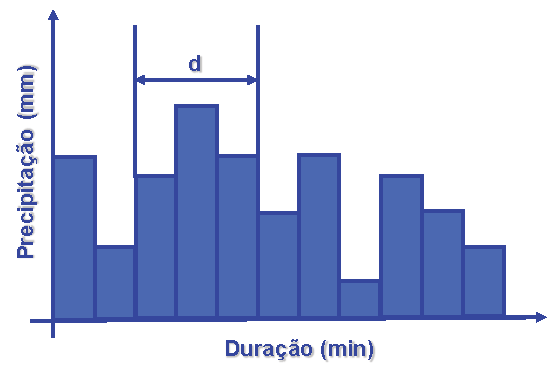
\includegraphics[width=0.7\textwidth]{Textuais/Figuras/desagregacao.pdf}
    \fonte{Autores}
    \label{fig:desagregacao}
\end{figure}

\subsection{Damé (2001)}

Para \citeonline{dame01} foram utilizados os parâmetros do modelo Bartlett-Lewis do Pulso Retangular Modificado (BLPRM) \cite{iturbe} e, como consequência, as séries de chuvas na duração de 15 minutos foram separadas de uma chuva com duração de 24 horas e implementadas no modelo de desagregação proposto por \citeonline{point-process}.

O modelo BLPRM considera como hipótese que a precipitação tenha estacionalidade mensal, ou seja, que suas propriedades estatísticas (média, variância, covariância, probabilidade de ocorrência de períodos secos) não se alterem dentro do mês. No trabalho de \cite{chuva-diaria} o método das relações (MR) foi utilizado para obter uma curva IDF histórica obtida por meio de dados pluviográficos para o mesmo período de anos; os resultados mostram que a IDF obtida pelo MR representou adequadamente a IDF histórica, levando os autores concluírem que este método é eficaz na desagregação da chuva diária. Dessa forma, é viável a possibilidade de usar esse método para obter relações de intensidade-duração-frequência em regiões nas quais se tenha pouco ou nenhuma informação pluviográfica e que existam abundantes registros de chuva diária.

Assumindo de que o método das relações foi eficaz na separação de chuvas diárias e que forneceu resultados próximos aos que seriam obtidos por meio do uso de plataforma de coleta de dados, verificou-se o desempenho das estimativas dos valores de intensidades máximas, quando se utiliza o método das relações para desagregar a chuva diária e estimar as relações IDF e assim chegar a uma conclusão sobre o método das relações.

\subsection{Bell (1969)}

De acordo com \citeonline{bell} estabeleceu relações experimentais entre chuvas com diferentes durações fundamentado em informações de séries fracionais de chuva observada nos EUA, Austrália, URSS, Porto Rico, Alasca, África do Sul e Havaí. O fundamento teórico desse estudo é a existência de similaridade entre a formação de chuvas. Devido a propriedades semelhantes em muitas partes do mundo devido a características de chuvas convectivas,  utiliza-se a equação de Bell para estimar a chuvas máximas entre os limites especificados. Devido a esse estudo ter sido realizado em diversas partes do mundo o trabalho de Bell apresenta algumas limitações. Devido aos valores adotados serem de várias regiões do mundo esses valores representam valores médios e não específicos de uma região; um outra limitação está na durações das chuvas, que devem estar entre 5 minutos e 120 minutos; pode- se, também destacar, como limitação ao método de Bell, a obrigatoriedade de se conhecer a precipitação máxima com duração de 60 minutos e intervalo de retorno de 10 anos, sendo necessário a coleta de dados por meio de pluviógrafos.

\citeonline{bell} utilizou dados de vários continentes e ajustou a Equação \ref{eq:bell}.

\begin{equation}
\label{eq:bell}
    P_{(t,T)} = (0,21 \times Ln(T) + 0,52)(0,54\times t^{0,25} -0,5) \times P_{(1,10)}
\end{equation}

Em que:

$P_{(t,T)}$ = Altura de chuva [mm]

T = Período de retorno [anos]

t = Tempo de duração [min]

$P_{(1,10)}$ = Altura de chuva com 1 hora de duração e período de retorno de 10 anos


\subsection{Chen (1983)}

\citeonline{rainfall} desenvolveu uma equação de IDF de chuvas que utiliza três alturas de precipitação: chuva de duração de 1 hora e tempo de retorno de 10 anos, chuva de 24 horas de duração e 10 anos de período de retorno e a chuva de 24 horas de duração e 100 anos de período de retorno. Neste estudo foi verificado que a partir da duração de 2 horas as relações de duração em relação a chuva de 24 horas variaram em função da relação da chuva de 1 hora e a de 24 horas.

A fórmula generalizada de \citeonline{rainfall} desenvolvida para as séries anuais, é dada pela Equação \ref{eq:chen1983}.

\begin{equation}
\label{eq:chen1983}
    P_{(t,T)} = \frac{a\times P(1,10)\times Log(10^{2-w}\times (Ln\frac{T_r}{T_r-1})^{1-w})}{(t+b)^c} \frac{t}{60}
\end{equation}

Em que:

P(t,T) = Altura de chuva com duração t e período de retorno $T_r$

$T_r$ = Período de Retorno [anos]

P(1,10) = Altura de chuva com 1 hora de duração e período de retorno de 10 anos

w = Relação entre a chuva de 1 hora de duração e período de retorno de 100 anos e a chuva de 1 hora de duração e período de retorno de 1 ano.

a, b,c = Obtidos em função da relação entre P(1,T) e P(24,T)


\section{Ajuste a distribuições de extremos estatísticas}

O desenvolvimento tecnológico e científico possibilita registrar o comportamento das variáveis hidrológicas, como por exemplo, chuvas, níveis de rios e nevascas. O acúmulo dos dados permitiu a criação de séries históricas, as quais são analisadas utilizando a estatística como uma ferramenta de tratamento de dados; dessa maneira o conhecimento dos conceitos estatísticos é indispensável ao desenvolvimento de estudos em hidrologia \cite{hidrologia-estatistica}.

As variáveis hidrológicas e hidrometerológicas têm sua variabilidade registrada por meio das chamadas séries temporais, as quais reúnem as observações ou medições daquela variável, organizadas de forma sequencial de sua ocorrência no tempo (ou espaço). Por limitações impostas pelos processos de medição ou observações, as variáveis hidrológicas, embora apresentem variações instantâneas são contínuas ao longo do tempo, ou do espaço, têm seus registros separados por determinados intervalos de tempo, ou de distância \cite{hidrologia-estatistica-np}.

De acordo com \citeonline{hidrologia-estatistica-np} as séries hidrológicas podem incluir todas as observações disponíveis, coletadas em intervalos de tempo regulares ao longo de vários anos de registros, ou apenas alguns de seus valores característicos como, por exemplo, os máximos anuais ou as médias mensais. 

Com o ajuste de um modelo de chuva diária baseando-se nos estudos de \citeonline{relacao-precipitacao} é possível aumentar a eficiência dos dados de chuvas, principalmente por conseguir a simulação e criação de extensas séries de precipitação, sendo estas, muitas vezes, maiores que as próprias séries de dados observados.

No caso específico de eventos hidrológicos extremos, como por exemplo máximos e mínimos, as séries reduzidas podem ser anuais, quando os registros consecutivos possuem o mesmo intervalo no tempo, ou de duração segmentada, em caso contrário.

As séries de máximos valores são empregadas para ajuste, segundo a lei probabilística que melhor descreva o processo, possibilitando extrapolações \cite{spchuva}.

Distribuições teóricas de probabilidade são simplesmente funções analíticas usadas para descrever o comportamento de determinadas variáveis. No caso de extremos, só os ajustes das séries longas em múltiplas localidades é que dá indicações sobre as distribuições que levam a melhor extrapolação \cite{piracicaba}.

Embora a teoria probabilística fundamental de valores extremos tenha sido desenvolvida há muito tempo, a modelagem estatística de extremos ainda permanece como assunto ativo de pesquisas dado seu importante papel nos projetos e gerenciamento de recursos hídricos, especialmente em um contexto de mudanças climáticas \cite{extremes}.

A teoria de valores extremos é fundamental nestes casos para a modelagem destes eventos. Os fundamentos desta teoria foram desenvolvidos por Fisher- Tippett (1928), que definiram os três tipos possíveis de distribuições assintóticas de valores extremos, conhecidas como de Gumbel (tipo I), Fréchet (tipo II) e Weibull (tipo III) \cite{ejgumbel}, que são casos especiais da Distribuição Generalizada de Valores Extremos desenvolvida por \citeonline{jen}. Além das distribuições de valores extremos, também são bastante utilizadas para descrever eventos raros as distribuições Log-normal e Pearson III \cite{sev}.

Diferentes distribuições, escolhidas entre as mais frequentemente utilizadas na descrição destas variáveis são consideradas, incluindo a de Gumbel, Log-Normal, Pearson III, Fréchet e Weibull, que tem, respectivamente, como funções de densidade de probabilidade acumulada.

\subsection{Distribuição de Gumbel}

Em geral, as distribuições de valores extremos de grandezas hidrológicas ajustam-se adequadamente à distribuição de Fisher- Tippett do tipo I, também nomeada como função de Gumbel \cite{hidro-aplicada}.

A distribuição de probabilidade de Gumbel é aplicada às séries históricas de valores extremos, especialmente, a precipitação máxima diária anual, sendo expressa pela Equação \ref{eq:gumbel}.

\begin{equation}
\label{eq:gumbel}
    P = 1 - e^{-e^{\gamma \times T_r}}
\end{equation}

A variável reduzida da distribuição de Gumbel é obtida pela aplicação da função de distribuição de frequência de Chow.

\begin{equation}
    \gamma_{Tr} = - Ln^{-Ln \left( 1 - \frac{1}{T_r} \right)}
\end{equation}

O evento extremo $X_Tr$ é representado pela Equação \ref{eq:evento-extremo}.

\begin{equation}
\label{eq:evento-extremo}
    X_{Tr} = \overline{x} + k_{Tr} \times s
\end{equation}

Em que:

$\overline{x}$ = Média dos valores extremos da série histórica

s = Desvio padrão amostral

$X_{Tr}$ = Evento extremo no decorrer do ano

\subsection{Distribuição de Fréchet}

A distribuição de Fréchet é uma forma particular da distribuição de valores extremos do Tipo II e de acordo com \citeonline{hidrologia-estatistica-np}, essa distribuição é conhecida também pela denominação Log-Gumbel, sendo pela Equação \ref{eq:frechet}.

\begin{equation}
\label{eq:frechet}
    P(x) = e^{-e^{-\alpha(x-\beta)}}
\end{equation}

No caso dos valores máximos, a distribuição de Fréchet refere-se à forma assintótica limite para um conjunto de N variáveis aleatórias originais, independentes e igualmente distribuídas conforme um modelo, de cauda superior polinomial. A distribuição foi usada pela primeira vez na análise de frequência de vazões de enchentes por Fréchet (1927), tendo, desde então, encontrado aplicações, como distribuição extrema de eventos hidrológicos máximos.

\subsection{Distribuição de Weibull}

Segundo \citeonline{catalunha} a distribuição de Weibull é utilizada em análise hidrológica para eventos extremos, sendo pouco conhecida a sua utilização em séries climáticas. Tem como principal método de ajuste de distribuição o da máxima verossimilhança, que consiste em determinar os valores de g e b pelas suas equações fundamentais.

A distribuição de Weibull a dois parâmetros tem como função de distribuição de probabilidades acumulada (FDA) a Equação \ref{eq:weibull}.

\begin{equation}
\label{eq:weibull}
    P(x) = 1 - e^{-(\frac{x-\alpha}{\beta})^\lambda}
\end{equation}

Em que:

$\alpha$ = Vida mínima ou Confiabilidade Intrínseca

$\lambda$ = Fator de forma (indica a forma da curva e a característica das falhas)

$\beta$ = Vida característica ou parâmetro de escala \\


\par \citeonline{catalunha} realizou um trabalho em Minas Gerais, concluindo que a distribuição de Weibull possui um ótimo desempenho para estimar as precipitações diárias.

\citeonline{chuvas-brasil}, realizando os primeiros estudos no Brasil, utilizou séries de valores extremos de precipitações de 98 plataformas de coleta de dados distribuídas em várias regiões do Brasil, para a construção de curvas IDF, utilizando com ferramenta estatística a distribuição de Weibull.

\subsection{Distribuição Log-Normal}

A distribuição Log-Normal tem como função de distribuição de probabilidades acumulada (FDA) a Equação \ref{eq:lognormal}.

\begin{equation}
\label{eq:lognormal}
    P(x) = \frac{1}{(x-a) \times \sqrt{2\pi\sigma^2}} \int_{-\infty}^{\infty} e^{-0,5} \left( \frac{Ln(x-a)-\mu}{\sigma^2} \right) dx
\end{equation}

A distribuição Log-Normal mostrou-se adequada para previsão das chuvas prováveis apenas nos meses de maiores intensidades segundo \citeonline{lavras}.

\section{Teste de Aderência}

De acordo com Oliveira (2003), a grande dificuldade com o desenvolvimento de modelos hidrológicos é a validação dos resultados obtidos, onde se deseja determinar indícios documentados que provem um alto grau de garantia a um processo específico, assegurando constantemente que os resultados estejam de acordo com a distribuição presentada para o conjunto de dados.

Diversos procedimentos estatísticos convencionais têm sido usados para este fim, tais como teste de comparação de médias (teste t), testes de comparação de variâncias (desvio padrão) como teste F, intervalos de confiança e outros diferentes níveis de probabilidade, e para a comparação de frequências de dados agrupados são normalmente utilizados os testes $X^2$ e Kolmogorov-Smirnov (OLIVEIRA, 2003).

O mesmo autor afirma que quando se ajusta uma distribuição de probabilidade a um conjunto de dados, trabalha- se com a hipótese de que a distribuição representa adequadamente aquele conjunto de informações.
Assim, Assis et al. (1996), comentam que em trabalhos de hidrologia, para se julgar a adequação do ajustamento dos dados observados a distribuição de frequência os testes estatísticos qui- quadrado ($x^2$) e o de Kolmogorov- Smirnov tem apresentado os melhores resultados.

\subsection{Qui-Quadrado}

O teste do $x^2$ é aplicado para verificar o ajuste de distribuição de probabilidade conhecida, no caso a gama, a uma amostra de dados de uma distribuição de probabilidade desconhecida. No teste do $x^2$ , a hipótese de nulidade admite que as frequências observadas se ajustem as frequências calculadas com a distribuição teórica (gama, exponencial, normal, Weibull) com seus parâmetros estimados com base nos dados amostrais. O valor de $x^2$ é dado pela Equação 16.

Se o valor do $x^2$  calculado é menor que o $$x^2 1 - a$$, k- p - 1 , sendo esse último proveniente de uma distribuição com GL = k – p - 1 graus de liberdade, sendo p o número de parâmetros estimados com base nos dados (p = 2, para o caso da distribuição gama) e a é o nível de significância estabelecido à hipótese de nulidade não é rejeitada e pode- se afirmar que os dados amostrais se aderem à distribuição teórica com um nível de significância a.

Catalunha et al (2002) em seu trabalho realizado em Minas Gerais aplicando cinco funções de densidade de probabilidade a séries de precipitação, concluíram que o teste do $x^2$  apresentou melhores características para verificar o ajuste de uma distribuição de probabilidade estimada a dados observados.

\begin{figure}
    \caption{Representação do qui quadrado}
    \centering
    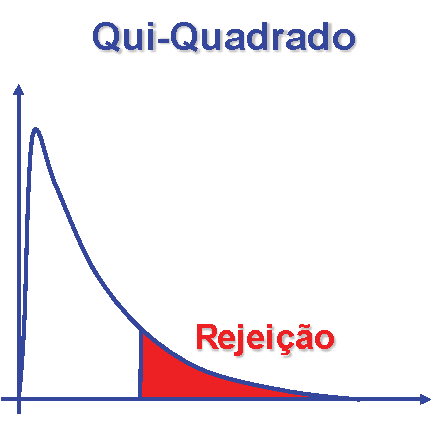
\includegraphics[width=0.5\textwidth]{Textuais/Figuras/qui-quadrado.pdf}
    \fonte{Autores}
    \label{fig:qui-quadrado}
\end{figure}

\subsection{Kolmogorov-Smirnov}

Esse teste é aplicado para verificar se os valores de uma certa amostra de dados podem ser considerados de uma população, com distribuição teórica pré-estabelecida.
Araújo et al (2001) utilizaram o teste de aderência de Kolmogorov- Smirnov a um nível de 5\% de probabilidade para verificar se o ajuste dos dados pluviométricos mensais se ajustam a função de distribuição de probabilidade normal e gama mista. O teste relaciona duas distribuições de frequências acumuladas, uma F’(x) teórica e outra F(x) derivada dos dados amostrais. O valor de Dmax é pela Equação 17

Caso o valor do Dmax observado é inferior ao Dmax obtido em tabelas, a um determinado nível de significância $\alpha$ , a hipótese de nulidade não é rejeitada, dessa forma, pode-se afirmar que os dados amostrais tem aderência à distribuição teórica.

\begin{figure}
    \caption{Representação kolmogorov}
    \centering
    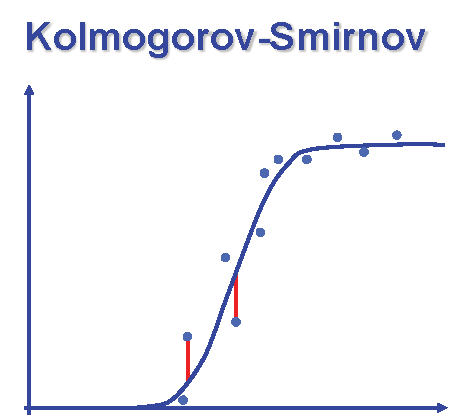
\includegraphics[width=0.5\textwidth]{Textuais/Figuras/kolmogorov.pdf}
    \fonte{Autores}
    \label{fig:kolmogorov}
\end{figure}

\section{Inteligência Artificial}

O termo aprendizado de máquina refere-se à detecção automatizada de padrões significantes em dados. Nas últimas décadas tem se tornado uma ferramenta comum em quase qualquer tarefa que requer informações extraídas de uma grande quantidade de dados \cite{uml}.

A ciência do aprendizado tem um importante papel em áreas como a estatística, mineração de dados e inteligência artificial, passando por áreas como engenharia, medicina, astronomia, robótica e outras disciplinas \cite{statistical-learning}.

Com o contínuo aumento de informações em forma digital, a necessidade de métodos automatizados para análise de dados continua crescendo. O objetivo do aprendizado de máquina é desenvolver métodos que possibilitam a detecção de padrões em dados, para futuramente reutilizá-los em forma de previsões em novos dados \cite{mlpp}. 

Dentre as ferramentas que integram a inteligência artificial destacam-se os Algoritmos Genéticos, Lógica Difusa e Redes Neurais Artificiais \cite{ai-fili}, sendo que este trabalho será focado em Redes Neurais Artificiais (RNA).

\section{Tipos de aprendizado}

O aprendizado depende da interação entre o ambiente e aprendiz. A primeira diferença consiste no aprendizado supervisionado e não supervisionado \cite{uml}.

\subsection{Aprendizado supervisionado}

O aprendizado supervisionado é aquele cujos parâmetros são pré-definidos e o algoritmo procura um padrão entre os dados. As informações que serão utilizadas para treinamento já contêm informações suficientes que permitem o algoritmo inferir uma relação entre uma ou múltiplas variáveis \cite{learning-algorithms}. A Figura \ref{fig:reg-linear} representa um exemplo de aprendizado supervisionado, a regressão linear.

\begin{figure}[h]
    \caption{Regressão linear é um exemplo de aprendizado supervisionado}
    \centering
    \includegraphics[width=0.5\textwidth]{Textuais/Figuras/linear-ml.png}
    \fonte{Adaptado de Russell e Norving (2010)}
    \label{fig:reg-linear}
\end{figure}

\subsection{Aprendizado não-supervisionado}

O aprendizado não supervisionado, permite abordar problemas com pouca ou nenhuma ideia de como deverá ser o resultado \cite{ai}. A rede tem de descobrir relações, padrões, regularidades ou categorias nos dados que lhe vão sendo apresentados e codificá-las em saídas. A Figura \ref{fig:nao-supervisionado} exemplifica o aprendizado não supervisionado: a classificação de dados em dois grupos.

\begin{figure}[h]
    \caption{(a) Distribuição da altura e peso de algumas pessoas. (b) Possível agrupamento de dados em 2 grupos}
    \centering
    \includegraphics[width=1.0\textwidth]{Textuais/Figuras/nao-supervisionado.png}
    \fonte{Adaptado de Murphy (2012)}
    \label{fig:nao-supervisionado}
\end{figure}

\subsection{Benefícios das RNA}

O poder de abstração das RNA deve-se à sua estrutura paralela e à capacidade de aprendizagem \cite{big-data}. A estrutura paralela resulta da existência de muitos neurônios ligados em uma mesma estrutura de pesos de conexão com facilidade de adaptação a distintos tipos entrada de dados. A estrutura paralela é desejável uma vez que permite a tolerância à falha, pois se algum neurônio falhar, os efeitos na rede como um todo não serão significativos para o desempenho da rede, dado que existe outro caminho de ligação entre os nós que pode iludir a falha \cite{statistical-learning}.

Uma das principais características das RNA é a capacidade de aprender por meio de exemplos e de generalização, ou seja, reconhecer padrões em elementos que não foram apresentados antes, possibilitando a produção de resultado aceitável oriundo de uma nova entrada de informação \cite{neural-network}.

As principais propriedades que podem se destacar das redes neurais artificiais são: não linearidade, mapeamento de entrada e saída, adaptabilidade e tolerância a falhas \cite{neural-network}.

\subsection{Redes Neurais Artificiais}

Redes neurais artificiais foram originalmente planejadas no meio do século 20 como um modelo computacional do cérebro humano. Sua aplicação era limitada devido a limitação computacional disponível na época, além de algumas questões teóricas que não foram solucionadas por várias décadas \cite{mlpp}.

É teorizado que devido a sua inspiração biológica, algoritmos baseados em redes neurais artificiais serão capazes de simular como o ser humano reconhece conceitos e objetos \cite{learning-algorithms}.

Em uma análise matemática, as RNA podem ser explicadas como uma mapeamento não linear de um vetor de espaço de entrada para um vetor de espaço de saída, que pode ser realizado por meio de camadas de funções de ativação, em que coordenadas de entrada são somadas de acordo com o valor de seus respectivos pesos e bias  para produzir uma saída simples, ativada ou não, de acordo com o respectivo nível de acionamento \cite{two-phase-flow}.

O conceito de rede neural artificial é basicamente introduzido pela biologia onde a rede neural tem um importante papel no ser humano. No corpo humano todo trabalho é realizado com ajuda da rede neural. Uma rede neural é uma cadeia de milhões de neurônios interconectados \cite{ann}.

\begin{figure}[h]
    \caption{Neurônios}
    \centering
    \includegraphics[width=0.7\textwidth]{Textuais/Figuras/neuronios.png}
    \fonte{Autores}
    \label{fig:neuronios}
\end{figure}

A terminologia rede neural é inspirada pelas operações biológicas realizadas por células especiais denominadas neurônios (Figura 5). Um neurônio é uma célula biológica especial que processa informação de um neurônio para outro com ajuda de um impulso elétrico e mudanças químicas que ocorrem no cérebro. Todo o processo de receber e enviar informação é realizado de uma forma particular: um neurônio recebe informações de outro neurônio através dos dendritos e envia informações com picos de atividade elétrica através de um longo e fino suporte conhecido como axônio que os divide em sinapses para enviá-los para outros neurônios \cite{ai}.

\begin{figure}[h]
    \caption{Célula de neuronio}
    \centering
    \includegraphics[width=0.7\textwidth]{Textuais/Figuras/celula.png}
    \fonte{Adaptado de Russell e Norving (2010)}
    \label{fig:celula}
\end{figure}

As redes neurais artificiais têm o seu equivalente ao neurônio denominado nó que recebe um conjunto de entradas ponderadas, processa a sua soma com as funções de ativação $\phi$, e passa o resultado da função de ativação para o próximo nó (Figura 7) até o término da rede (Equação \ref{eq:no}) \cite{ann}.

\begin{equation}
\label{eq:no}
    \phi \left( \sum_{i} w_i\times a_i \right) = \phi(w^T\times a)
\end{equation}

Visualmente é equivalente a Figura \ref{fig:neuronio-rna}.

\begin{figure}[h]
    \caption{Representação de um neurônio na RNA}
    \centering
    \includegraphics[width=0.4\textwidth]{Textuais/Figuras/rep-neronio.png}
    \fonte{http://briandolhansky.com/blog/artificial-neural-networks-linear-regression-part-1}
    \label{fig:neuronio-rna}
\end{figure}

\subsection{Funções de ativação}

Funções de ativação são basicamente funções de transferência que são geradas pelos neurônios artificiais e envia sinal para outro neurônio artificial \cite{ann}. As funções de ativação mais comuns são: Limiar, Degrau, Degrau Unitário, Linear e Logística (Figura \ref{fig:neuronio-rna}). 

\begin{figure}[h]
    \caption{Funções de ativação}
    \centering
    \includegraphics[width=0.8\textwidth]{Textuais/Figuras/funcao-ativacao.png}
    \fonte{https://pt.stackoverflow.com/questions/61187/como-implementar-a-camada-oculta-em-uma-rede-neural-de-reconhecimento-de-caracte}
    \label{fig:neuronio-rna}
\end{figure}

Existem diversas funções de ativação, como por exemplo a função linear (Equação \ref{eq:linear}), também denominada função identidade.

\begin{equation}
\label{eq:linear}
    \phi(w^Ta) =w^Ta
\end{equation}

Outra função de ativação é a função sigmoid (Logística) representada pela Equação \ref{eq:sigmoid}.

\begin{equation}
\label{eq:sigmoid}
    \phi(w^Ta)=\frac{1}{1+exp(-w^Ta)} 
\end{equation}

Uma função muito utilizada é a tanh, representada pela Equação \ref{eq:tanh}.

\begin{equation}
\label{eq:tanh}
    \phi(w^Ta) = tanh(w^Ta)
\end{equation}

A possível criação de uma rede neural ocorre por meio do encadeamento dos nós. Usualmente esse processo é realizado utilizando camadas, as saídas de um nó estão conectadas a entrada dos nós da próxima camada \cite{tensor-flow}.

O objetivo de aproximações de funções é treinar uma rede neural que seja capaz, a partir de um conjunto de dados entrada-saída, de mapear uma determinada relação funcional que contemple o universo de amostras sob análise. O treinamento, nesse caso, envolve o aprendizado dos pesos de borda corretos para produzir a saída de destino, dada uma entrada \cite{uml}. A rede e seus pesos treinados formam uma função (denominada h) que operam sob dados de entrada. Com a rede treinada, é possível produzir previsões para valores de entrada previamente desconhecidos.

É possível treinar uma rede neural para realizar regressão ou classificação. Nesse trabalho iremos abordar somente a regressão linear. 

\begin{figure}
    \caption{Representação de uma regressão e classificação}
    \centering
    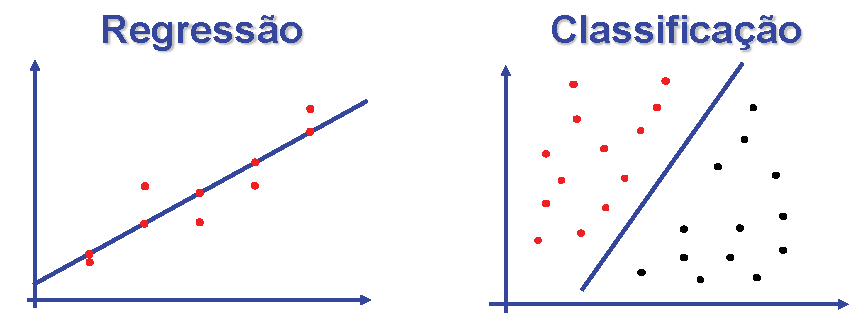
\includegraphics[width=0.8\textwidth]{Textuais/Figuras/ai.pdf}
    \fonte{Autores}
    \label{fig:reg-class}
\end{figure}

\subsection{Regressão Linear}

Regressão linear é a forma mais simples de regressão \cite{ai}. Modelamos o nosso sistema como combinações lineares de features para produzir uma saída.

\begin{equation}
    y_i = h(x_i,w) = w^Tx_i
\end{equation}

A RNA torna-se responsável por encontrar os pesos que geram o melhor resultado para os dados de treinamento. Um modo de verificar a qualidade da aproximação é utilizando o método dos mínimos quadrados (também conhecido como Loss) \cite{tf}.

\begin{equation}
    L(w) = \sum_i \left( h(x_i,w)-y_i^2 \right)^2
\end{equation}

Para poder realizar o melhor ajuste é preciso minimizar o valor de L(w). Esse método possui uma solução analítica, mas em geral pode-se resolver utilizando o método do gradiente descendente \cite{ai}.

A rede neural mais simples utiliza o método dos mínimos quadrados para realizar uma regressão linear como mostra a Figura 10. 

Essa rede recebe como entrada de dados duas features xi(1) e xi(2), os pesos das features como w1 e w2 e os soma, e como saída tem-se a previsão yi. Pode-se considerar uma rede neural com n parâmetros de entrada, porém a rede deve conter n pesos, sendo equivalente um peso para cada entrada. Para poder determinar a qualidade de aproximação é possível utilizar o método dos mínimos quadrados \cite{ML}.

\citeonline{tensor-flow} utiliza o método do gradiente descente para minimizar os erros em relação aos dados de treinamento. Primeiramente deriva-se o gradiente descendente em relação a um determinado peso wj->k

Nesse ponto, calcula-se o gradiente da função da rede em relação ao peso da derivada parcial. 

A função da rede é dada pela Equação \ref{eq:funcao-rede}.

\begin{equation}
\label{eq:funcao-rede}
    h(x_i,w) = w_1x_i^{(1)} + w_2x_i^{(2)}
\end{equation}

O gradiente em relação a w1 é apenas x1, e o gradiente em relação a w2 é apenas x2, dessa forma o gradiente é dado pela Equação \ref{eq:gradiente}.

\begin{equation}
\label{eq:gradiente}
    \nabla_wL(w) = \left( \frac{\partial L(w)}{\partial w_1}, \frac{\partial L(w)}{\partial w_2} \right) = \left( \sum_i 2x_i ^{(1)} h(x_i,w), \sum_i 2x_i ^{(2)} h(x_i,w) \right)
\end{equation}

Agora é possível atualizar os pesos utilizando o gradiente descendente padrão

\begin{equation}
    w = w -\eta \nabla_w L(w)
\end{equation}

Onde ``$\eta$`` é o passo.

\subsection{Testando a RNA}

Com a rede treinada, testar consiste em obter a previsão para cada ponto xi utilizando a função h(xi, w). O erro pode ser calculado da mesma forma do treinamento utilizando a Equação \ref{eq:teste-rna}.

\begin{equation}
\label{eq:teste-rna}
    L(w) = (\overline{y_i} - y_i)^2
\end{equation}

\subsection{Teorema Universal da Aproximação}

O Teorema Universal da Aproximação garante que uma Rede Neural Artificial do tipo Função Radial de Base pode ser treinada para ajustar, satisfatoriamente, qualquer função contínua definida em um conjunto fechado \cite{neural-network}.